\section{Distribution and Documentation}

The gemc framework is documented on the gemc website \cite{gemc}. This includes the latest news and releases,
examples, procedure details and all options documentation.

The software is distributed in two ways: with docker, or by downloading the source from the its public repository.

\subsubsection{Docker}

A docker container with the necessary libraries to run GEMC and the reconstruction software
is created in the JeffersonLab hub repository \cite{jlabDocker}


The container is tagged, and every tag contains a set version of these libraries:

\begin{itemize}
	\item event generators such as generate-dis, dvcsgen generator executables
	\item gemc with the clas12 geometry
	\item CLARA
	\item Coatjava
\end{itemize}

Collaborators access these containers and all the software inside by using the command:

\begin{lstlisting}[language=Python]
docker run -it --rm jeffersonlab/clas12simulations:iprod bash
\end{lstlisting}

The only requirement is the docker app, avaialble in Windows, Mac and Linux OS flavors.


\subsubsection{Source Code Dowload}

The code repository is \url{https://github.com/gemc/source}. To compile GEMC several libraries are needed:

\begin{itemize}
	\item clhep: Class Library for High Energy Physics \cite{clhep}
	\item xercesc: validating XML parser \cite{xercesc}
	\item geant4: the libraries to simulate the passage of particles through matter \cite{geant4}
	\item qt: a C++ graphic library \cite{qt}
	\item evio: the CLAS12 data format \cite{evio}
	\item CCDB: the calibration database based on mysql \cite{ccdb}
\end{itemize}


\subsubsection{Documentation and code repository}

The main documentation is on the gemc website \cite{gemc}. It includes example on how to create and run custom geometry
and use various features like generators, geometry factories, hit definitions, output, etc.

The code is kept on the guthub repository \url{https://github.com/gemc/source}. Gemc is released on a semi-annual cycle.

\subsubsection{Clas12 Tags}
The CLAS12 development of both hit process routines and geometry is kept in a separate repository, \url{https://github.com/gemc/clas12Tags},
that also contains documentation on how to run with configurations corresponding to the various experiment, how to change the
beamline configuration, and switch between code and geometry releases.


\subsubsection{Contribution to code and geometry}

The code repository is public. The development contributions mechanism is illustrated in \F{github}: collaborators fork the repository
and make pull request that are validated by the code author.

\begin{figure}
	\centering
	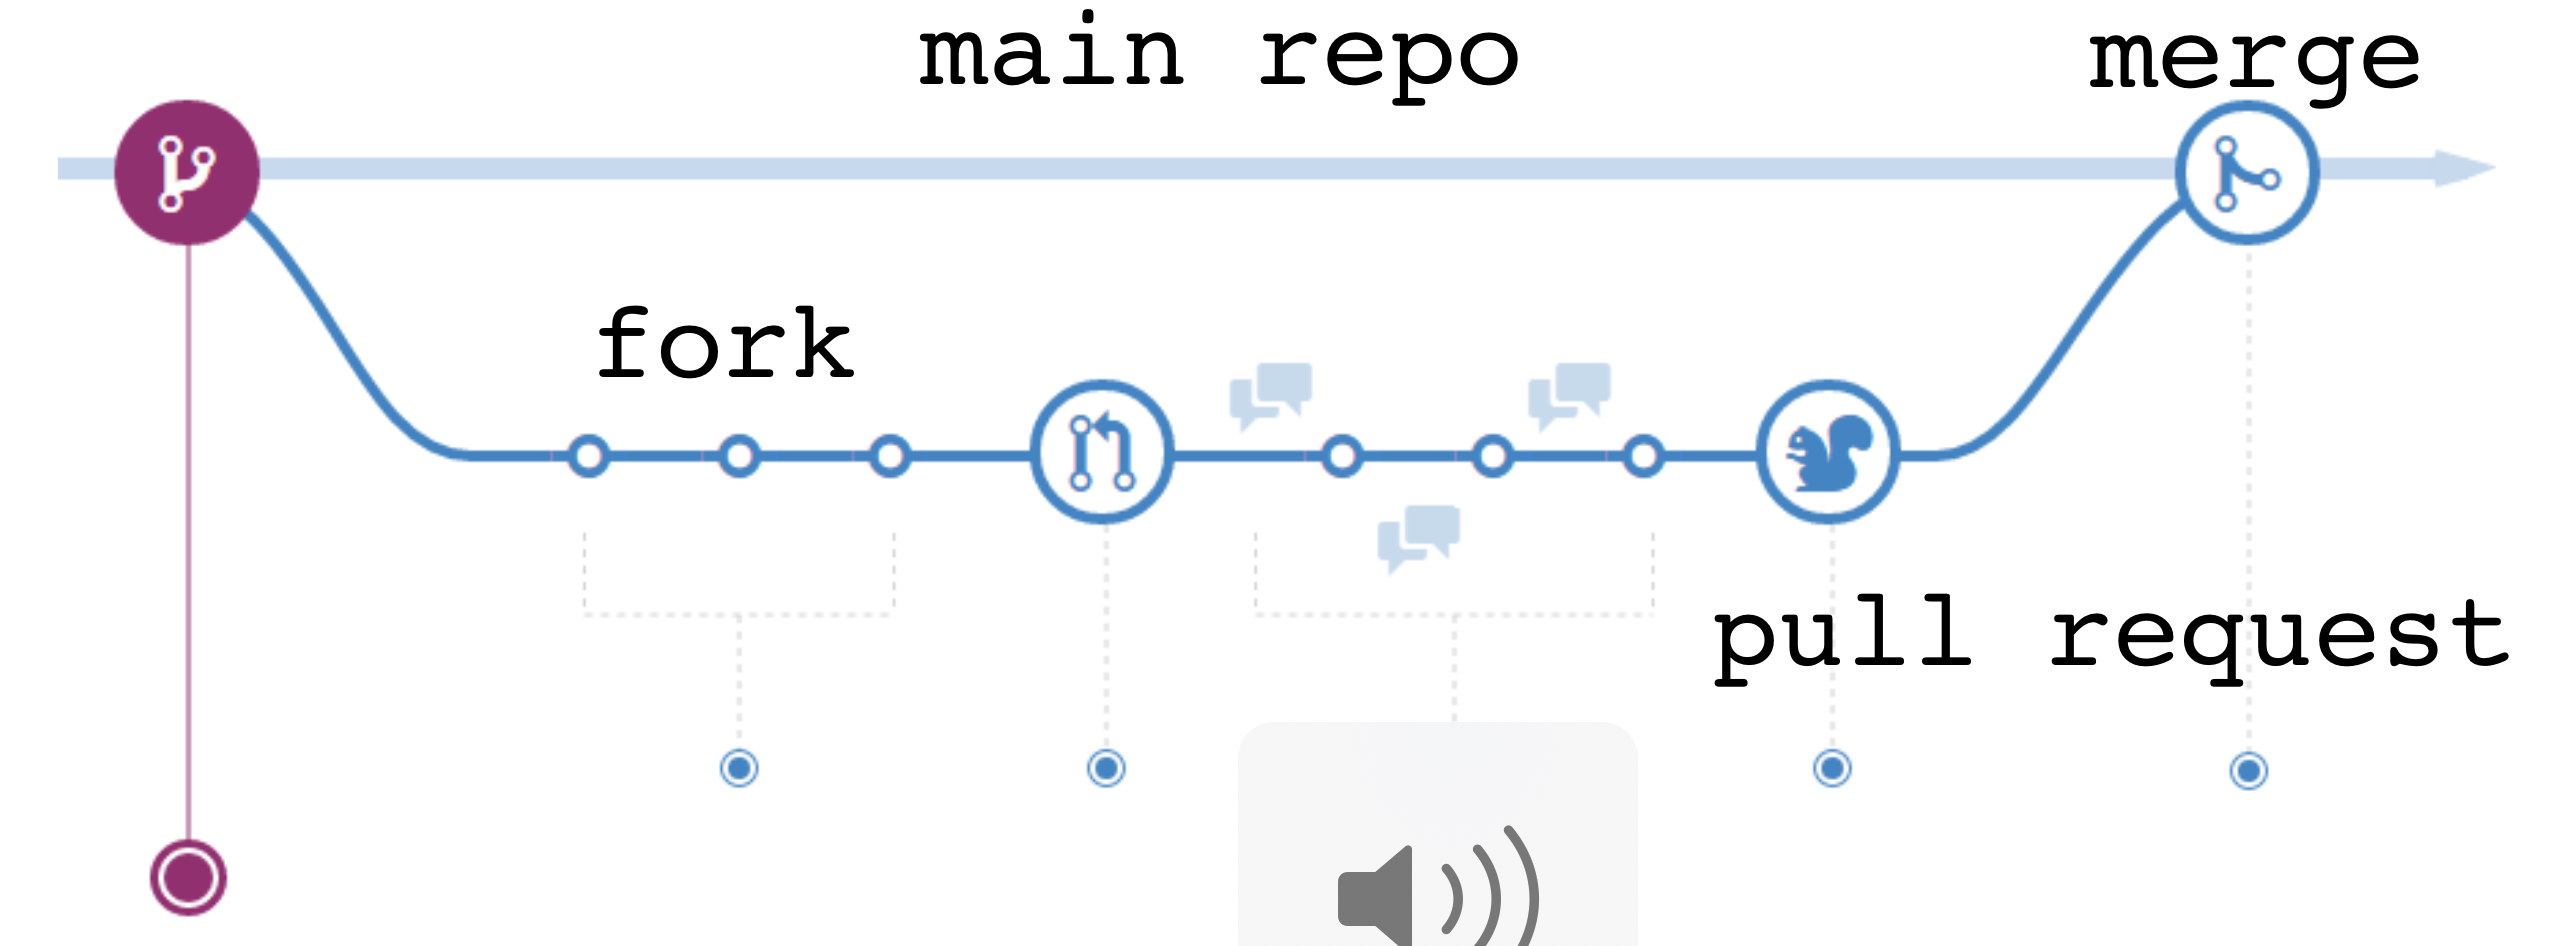
\includegraphics[width=0.95\columnwidth,keepaspectratio]{img/github.png}
	\caption{Typical workflow of contribution to the code: the main repository is forked and worked on. During the process comments
             can be made part of the development process. When the users make the pull request, the changes are validated and then merged
             to the master repository, or sent back with comments if there were problems.}
	\label{fig:github}
\end{figure}




